% Supplementary Figure 5 -- primary layer-specific modelling workflow.
%
% Step text is reproduced verbatim from the figure this replaces; only the
% drawing is new. The figure carries no title, subtitle or footnote: those
% belong to the caption in supp.tex, not to the artwork. See workflow-style.tex for the shared styling.
%
% Build with code/latex_workflow/run_all.sh (do not run pdflatex here by hand:
% the script is what puts the PDF where results/figures expects it).

\documentclass[border=6mm]{standalone}
% Shared house style for the workflow schematics.
%
% Both supplementary workflow figures are the same kind of diagram: a titled
% header, a numbered chain of steps that wraps onto a second row, and a closing
% note. Everything about how that looks lives here, so the two figure files are
% content only and cannot drift apart visually.
%
% Included by the figure files; not a standalone document.

\usepackage[T1]{fontenc}
\usepackage{lmodern}
\usepackage{tikz}
\usetikzlibrary{arrows.meta, positioning, calc}

% --- palette ---------------------------------------------------------------
% One accent per step role, dark enough to stay legible in greyscale. Header
% bars carry the accent at full strength; bodies carry an 8% tint of it.
\definecolor{wfInk}{HTML}{1F2D3D}      % body text
\definecolor{wfMuted}{HTML}{5A6B7B}    % secondary text, arrows
\definecolor{wfRule}{HTML}{C7D0D9}
\definecolor{wfSetup}{HTML}{B07D2B}    % scope-setting steps
\definecolor{wfFit}{HTML}{2E6DA4}      % fitting and prediction steps
\definecolor{wfInner}{HTML}{2E7D52}    % nested-resampling steps

% --- geometry --------------------------------------------------------------
% One box width drives everything; the header and body derive their text widths
% from it so the two nodes are exactly the same total width and align on their
% north-west corners.
\newlength{\wfBoxW}   \setlength{\wfBoxW}{52mm}
\newlength{\wfBoxH}   \setlength{\wfBoxH}{42mm}
\newlength{\wfPad}    \setlength{\wfPad}{2.6mm}
\newlength{\wfTextW}  \setlength{\wfTextW}{\dimexpr\wfBoxW-2\wfPad\relax}
\newlength{\wfHeadH}  \setlength{\wfHeadH}{7.4mm}
\newlength{\wfGapX}   \setlength{\wfGapX}{7mm}
% Five boxes and four gaps: the row-1 chain sets the canvas width, which the
% title and footnote blocks then span.
\newlength{\wfCanvasW}\setlength{\wfCanvasW}{\dimexpr 5\wfBoxW+4\wfGapX\relax}

% Resize the step boxes. The tikz styles read \wfTextW and \wfBoxH when a node
% is created, so setting these before a \wfstep call changes that box and every
% later one until it is set again. Row 2 uses wider, shorter boxes because its
% steps carry more text and there are only two of them.
\newcommand{\wfsetbox}[2]{%
  \setlength{\wfBoxW}{#1}%
  \setlength{\wfBoxH}{#2}%
  \setlength{\wfTextW}{\dimexpr\wfBoxW-2\wfPad\relax}%
}

\tikzset{
  wfbody/.style={
    draw=#1, fill=#1!8, line width=0.5pt, rounded corners=1.8pt,
    text width=\wfTextW, minimum height=\wfBoxH, inner xsep=\wfPad,
    inner ysep=0pt, align=left, anchor=north west,
  },
  wfhead/.style={
    fill=#1, text=white, text width=\wfTextW, inner xsep=\wfPad,
    inner ysep=1.9mm, align=left, anchor=north west, rounded corners=1.8pt,
    font=\sffamily\bfseries\small,
  },
  wfarrow/.style={
    -{Stealth[length=2.4mm, width=1.7mm]}, draw=wfMuted, line width=0.8pt,
  },
}

% \wfstep{<accent>}{<node name>}{<placement>}{<number>}{<title>}{<body>}
%
% The body node is drawn first and reserves the header's height at the top; the
% header bar is then laid over that reserved strip. Body text is a text width,
% so paragraphs wrap themselves and every box keeps the same footprint no matter
% how much text a step carries.
% The header height is reserved with a zero-width strut rather than \vspace*:
% inside a TikZ node with align=left the content starts in horizontal mode, so
% a leading \vspace* is applied after the first line has already been set and
% the header then covers that line. A strut forces a line box of exactly the
% header's height, whatever mode we are in.
\newcommand{\wfstep}[6]{%
  \node[wfbody=#1, #3] (#2) {%
    \rule{0pt}{\dimexpr\wfHeadH+2.2mm\relax}\par
    \color{wfInk}\sffamily\fontsize{7.6}{10}\selectfont\raggedright #6%
  };%
  \node[wfhead=#1] at (#2.north west) {#4\hspace{1.4ex}#5};%
}

% A step body is a list of short statements; \wfsep separates them.
\newcommand{\wfsep}{\par\vspace{1.5mm}}

% \wftitle{<title>}{<subtitle>}
\newcommand{\wftitle}[2]{%
  {\color{wfInk}\sffamily\bfseries\fontsize{17}{20}\selectfont #1\par}%
  \vspace{1.8mm}%
  {\color{wfMuted}\sffamily\fontsize{9}{11}\selectfont #2\par}%
  \vspace{2.8mm}%
  {\color{wfRule}\rule{\linewidth}{0.6pt}}%
}

% \wffoot{<note>}
\newcommand{\wffoot}[1]{%
  {\color{wfRule}\rule{\linewidth}{0.6pt}}\par\vspace{1.9mm}%
  {\color{wfMuted}\sffamily\itshape\fontsize{7.8}{9.6}\selectfont #1\par}%
}


\begin{document}
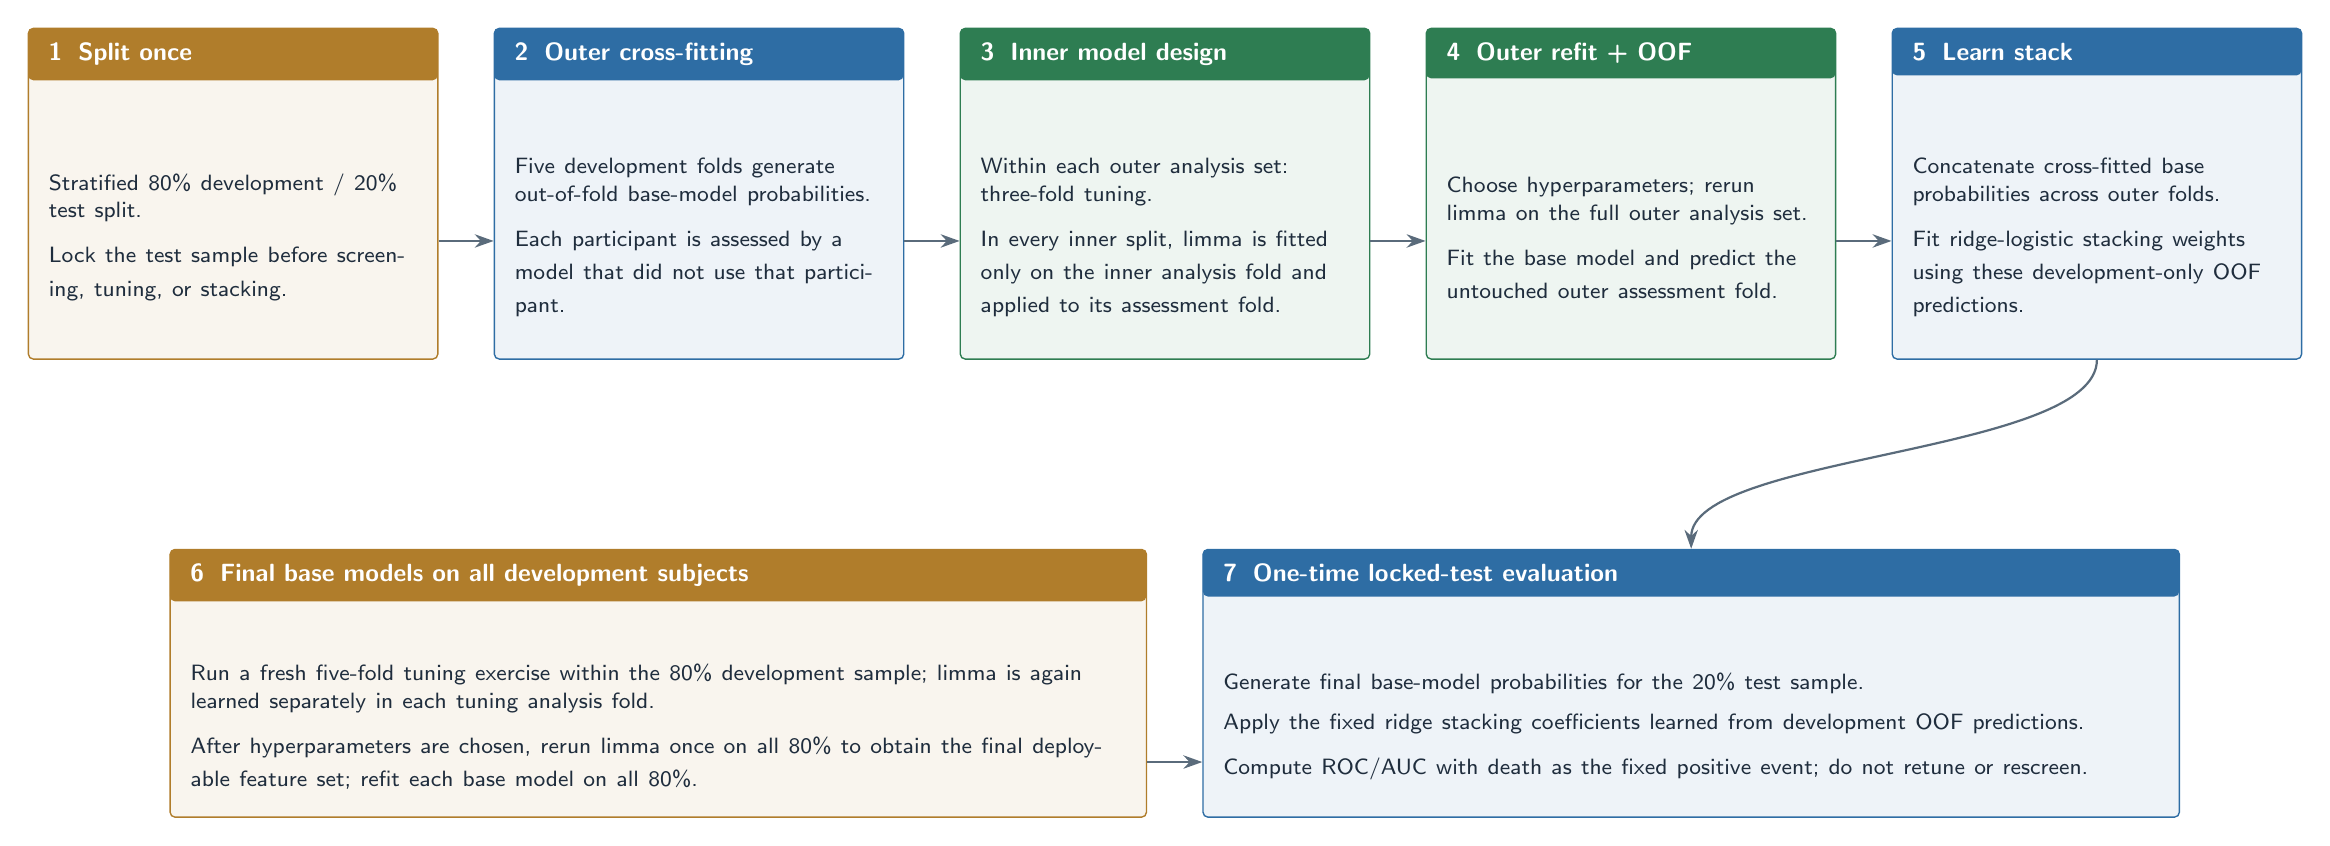
\begin{tikzpicture}[node distance=0pt]

% Row 1 -------------------------------------------------------------------
\wfstep{wfSetup}{s1}{at={(0,0)}}{1}{Split once}{%
  Stratified 80\% development / 20\% test split.\wfsep
  Lock the test sample before screening, tuning, or stacking.}

\wfstep{wfFit}{s2}{at={($(s1.north east)+(\wfGapX,0)$)}}{2}{Outer cross-fitting}{%
  Five development folds generate out-of-fold base-model probabilities.\wfsep
  Each participant is assessed by a model that did not use that participant.}

\wfstep{wfInner}{s3}{at={($(s2.north east)+(\wfGapX,0)$)}}{3}{Inner model design}{%
  Within each outer analysis set: three-fold tuning.\wfsep
  In every inner split, limma is fitted only on the inner analysis fold and
  applied to its assessment fold.}

\wfstep{wfInner}{s4}{at={($(s3.north east)+(\wfGapX,0)$)}}{4}{Outer refit + OOF}{%
  Choose hyperparameters; rerun limma on the full outer analysis set.\wfsep
  Fit the base model and predict the untouched outer assessment fold.}

\wfstep{wfFit}{s5}{at={($(s4.north east)+(\wfGapX,0)$)}}{5}{Learn stack}{%
  Concatenate cross-fitted base probabilities across outer folds.\wfsep
  Fit ridge-logistic stacking weights using these development-only OOF
  predictions.}

% Row 2 -------------------------------------------------------------------
% Two steps rather than five, each carrying more text: wider and shorter.
\wfsetbox{124mm}{34mm}

\wfstep{wfSetup}{s6}{at={($(s1.south west)+(18mm,-24mm)$)}}{6}{Final base models on all development subjects}{%
  Run a fresh five-fold tuning exercise within the 80\% development sample;
  limma is again learned separately in each tuning analysis fold.\wfsep
  After hyperparameters are chosen, rerun limma once on all 80\% to obtain the
  final deployable feature set; refit each base model on all 80\%.}

\wfstep{wfFit}{s7}{at={($(s6.north east)+(\wfGapX,0)$)}}{7}{One-time locked-test evaluation}{%
  Generate final base-model probabilities for the 20\% test sample.\wfsep
  Apply the fixed ridge stacking coefficients learned from development OOF
  predictions.\wfsep
  Compute ROC/AUC with death as the fixed positive event; do not retune or
  rescreen.}

% Flow --------------------------------------------------------------------
\foreach \a/\b in {s1/s2, s2/s3, s3/s4, s4/s5}{%
  \draw[wfarrow] ($(\a.east)+(0,-6mm)$) -- ($(\b.west)+(0,-6mm)$);
}
\draw[wfarrow] (s5.south) .. controls ($(s5.south)+(0,-12mm)$) and
  ($(s7.north)+(0,12mm)$) .. (s7.north);
\draw[wfarrow] ($(s6.east)+(0,-10mm)$) -- ($(s7.west)+(0,-10mm)$);

\end{tikzpicture}
\end{document}
